\documentclass[12pt, twoside]{article}
\usepackage[francais]{babel}
\usepackage[T1]{fontenc}
\usepackage[latin1]{inputenc}
\usepackage[left=5mm, right=5mm, top=5mm, bottom=5mm]{geometry}
\usepackage{float}
\usepackage{graphicx}
\usepackage{array}
\usepackage{multirow}
\usepackage{amsmath,amssymb,mathrsfs}
\usepackage{soul}
\usepackage{textcomp}
\usepackage{eurosym}
 \usepackage{variations}
\usepackage{tabvar}


\pagestyle{empty}

\begin{document}




\section*{\center{Devoir maison 4}}


\bigskip





\fbox{

\begin{minipage}{18cm}
\textit{Devoir � rendre pour le \textbf{vendredi 28 janvier 2012}. La
pr�sentation et la clart� sont not�es sur 1 point. Les exercices 1 et 2 se font
sur la photocopie, les autres sur votre feuille.}
\end{minipage}
}


\bigskip


\ul{Exercice 1}: (\textit{4,5 points}) 

\begin{tabular}{cc}
\begin{minipage}{11cm}
\begin{enumerate}
  \item Coder sur la figure l'angle $\widehat{zHx}$ en rouge, l'angle
  $\widehat{BGH}$ en vert et l'angle $\widehat{JEH}$ en bleu.
  \item Quels autres noms peut-on donner � l'angle $\widehat{GBH}$? Donner
  quatre solutions.
  
  \ldots \ldots \ldots \ldots \ldots \ldots \ldots \ldots \ldots \ldots \ldots
  \ldots \ldots \ldots \ldots \ldots \ldots \ldots
  \item Les angles $\widehat{HIE}$ et $\widehat{JIB}$ ont m�me mesure. Coder la
  figure.
  \end{enumerate}
\end{minipage} 
&
\begin{minipage}{7cm}

\qquad 
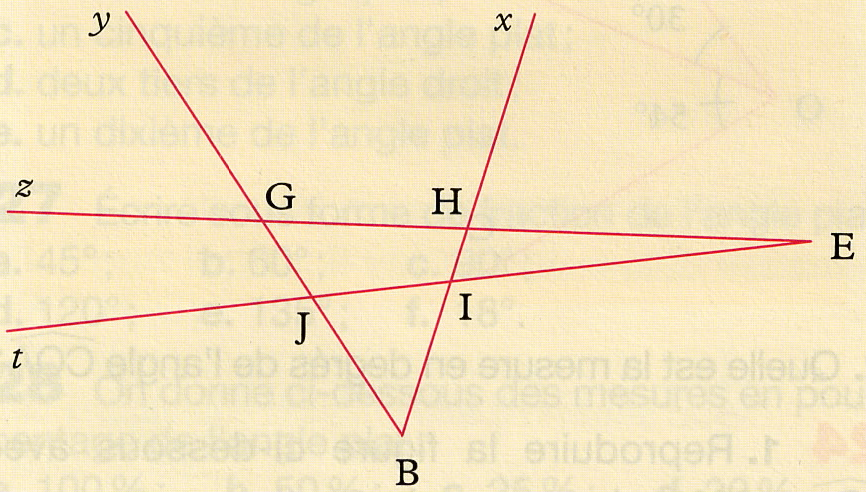
\includegraphics[width=67mm]{images/ex1.png}

\end{minipage}
\end{tabular}


\bigskip


\ul{Exercice 2}: (\textit{4,5 points})


\enskip

A l'aide de la figure, compl�ter le tableau suivant:


\begin{tabular}{cc}
\begin{minipage}{12cm}
\begin{tabular}{|c|c|c|c|}
\hline


angle & nom de l'angle & 
\begin{minipage}{3,1cm}
aigu, obtus, droit ou plat
\end{minipage} &
\begin{minipage}{3,1cm}
mesure de l'angle (au rapporteur)
\end{minipage}

\\

\hline

1 & & & \\

\hline

2 & & & \\

\hline

3 & & & \\

\hline

4 & & & \\

\hline

5 & & & \\

\hline

6 & & & \\

\hline


\end{tabular}
\end{minipage}
&
\begin{minipage}{68mm}
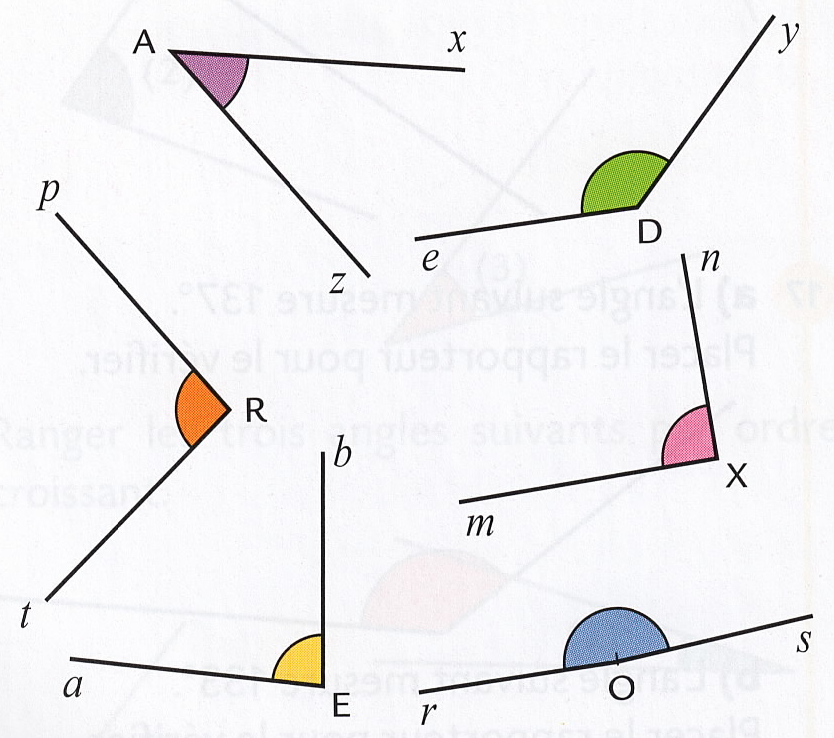
\includegraphics[width=68mm]{images/ex2.png}
\end{minipage}
\end{tabular}

\bigskip


\ul{Exercice 3}: (\textit{2,5 points})

\begin{tabular}{cc}
\begin{minipage}{14cm}
A l'aide des codages indiqu�s, calculer la mesure de l'angle $\widehat{NDE}$
(justifiez votre r�ponse).
\end{minipage}
&
\begin{minipage}{4cm}

\qquad 
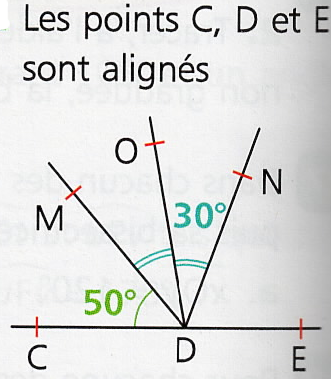
\includegraphics[width=3cm]{images/ex3.png}
\end{minipage}
\end{tabular}

 
\bigskip


\ul{Exercice 4}: (\textit{2,5 points})

\enskip

\begin{tabular}{cc}
\begin{minipage}{14cm}
La figure ci-contre est un sch�ma � main lev�e. Les points U, L et M sont-ils
align�s. Expliquer pourquoi (il faut effectuer un calcul pour expliquer votre
r�ponse).
\end{minipage}
&
\begin{minipage}{35mm}
\quad
\end{minipage}
\end{tabular}


\bigskip


\ul{Exercice 5}: (\textit{5 points})


\begin{enumerate}
  \item Tracer une droite (d), puis placer sur (d) trois points distincts A, B
  et C align�s dans cet ordre.
  \item Placer un point D tel que $\widehat{ABD}$=120� et BD=4cm.
  \item Calculer la mesure de l'angle $\widehat{CBD}$ (�crivez votre calcul).
  \item Placer un point E tel que la demi-droite [BE) soit la bissectrice de
  l'angle $\widehat{ABD}$.
  \item Montrer que la demi-droite [BD) est la bissectrice de l'angle
  $\widehat{EBC}$.
\end{enumerate}
\end{document}
